% EE4525 2025/2026 — A Residue Amplifier for a Pipeline ADC — final report
% Template adapted from the EE4520 HW2 report (from-ee4520/HW2_EE4520_5714699/main.tex).
% STRUCTURE IS COMPULSORY (project PDF p.11): Title, D1 table, D2 node-V, D3 branch-I,
%   D4 settling plot, D5 noise plot, D6 FoM comparison, then the Short Explanation (page 8).
% Fill the Achieved column + the figures (see ../analysis/09_simulation_runbook.md and
%   report/README.md for how to extract each figure). Submit PDF named [StudentNumber].pdf.
\documentclass{article}
\usepackage{graphicx}
\usepackage{amsmath}
\usepackage{booktabs}
\usepackage{siunitx}
\usepackage{float}

% Compile-ready placeholder box — replace each with the real \includegraphics line above it.
\newcommand{\fig}[1]{\fbox{\parbox[c][0.32\textheight][c]{0.92\textwidth}{\centering\itshape%
  [Figure placeholder --- #1. Replace with \texttt{\textbackslash includegraphics}.]}}}

\title{EE4525 2025/2026 -- A Residue Amplifier for a Pipeline ADC}
\author{Daniel Tyukov \\ Student Number: 5714699 \\ Electrical Engineering, TU Delft}
\date{June 2026}

\begin{document}

\maketitle
\tableofcontents
\clearpage

% ============================== DELIVERABLE 1 ==============================
\section{Deliverable 1 -- Table of Results}
% Hard specs (green-shaded in the PDF) are \textbf{bold}: rows 1--4, 8, 9, 13, 14, 17.
% Fill the Achieved column. FoM_dB uses the NEGATIVE sign (gives a positive dB).
\begin{table}[H]
\centering
\small
\begin{tabular}{@{}c l l l l@{}}
\toprule
\# & Design Item & Unit & Spec & Achieved \\
\midrule
1  & SNR & [dB] & \textbf{66} & \\
2  & $A\beta_{\text{settle}}$ (loop setting) & [dB] & \textbf{66} & \\
3  & $A_{\text{settle}}$ (amplifier settling) & [dB] & \textbf{$>78$} & \\
4  & $T_{\text{settle}}$ (to required accuracy) & [ns] & \textbf{25} & \\
5  & $T_{30\text{dB}}$ & [ns] & --- & \\
6  & $T_{38.6\text{dB}}$ & [ns] & --- & \\
7  & $\tau = T_{38.6\text{dB}} - T_{30\text{dB}}$ & [ns] & --- & \\
8  & Power dissipation (amplifiers only) & [mW] & \textbf{$<3$}, low as poss. & \\
9  & $I(V_{dd})$ (amplifiers only, no biasing) & [mA] & \textbf{$<1.7$}, low as poss. & \\
10 & Total effective $kT/C$ noise at output & [$\mu$V$_{\text{rms}}$] & free & \\
11 & Total integrated amplifier noise & [$\mu$V$_{\text{rms}}$] & free & \\
12 & Total integrated noise (10\,kHz--100\,GHz) & [$\mu$V$_{\text{rms}}$] & free & \\
13 & Input step voltage & [mV] & \textbf{Output/4} & \\
14 & Output step voltage & [V] & \textbf{free} & \\
15 & $C_{in}$ & [pF] & --- & \\
16 & $C_{fb}$ & [pF] & --- & \\
17 & $C_{load}$ & [pF] & \textbf{$= C_{in}$} & \\
18 & $C_{CM}$ & [pF] & --- & \\
19 & $R_{fb}$ & [G$\Omega$] & big & \\
20 & $C_{big}$ & [nF] & big & \\
21 & FoM$_{lin}=2\pi\cdot$Power$\cdot\tau\,/\,$SNR$_{lin}^2$ & [J] & & \\
22 & FoM$_{dB}=-10\log_{10}(\mathrm{FoM}_{lin})$ & [dB] & $>170$ & \\
\bottomrule
\end{tabular}
\end{table}

\noindent\textit{Design choices (see \texttt{analysis/01\_specs\_and\_budget.md}):} residue gain
$C_{in}/C_{fb}=4$ ($\Rightarrow C_{in}:C_{fb}=4{:}1$, $\beta=C_{fb}/(C_{in}+C_{fb})=1/5$,
noise gain $5$); $C_{load}=C_{in}$; output common-mode $0.9$\,V.

\subsection*{Computation notes}
\begin{itemize}
\item SNR: $\mathrm{SNR}_{dB}=20\log_{10}(V_{sig,rms}/V_{n,tot,rms})$, with
      $V_{n,tot}=\sqrt{V_{n,amp}^2+V_{n,kT/C}^2}$ (amplifier noise + hand-computed $kT/C$).
\item $\tau$: $\tau=T_{38.6\text{dB}}-T_{30\text{dB}}$ (one $e$-fold $=8.6$\,dB).
\item Power: $P=\overline{I(V_{dd})}\cdot 1.8~\mathrm{V}$ (biasing on a separate $V_{ddb}$, excluded).
\item FoM: linear $<9.5\times10^{-18}$\,J $\Leftrightarrow$ FoM$_{dB}>170$.
\end{itemize}
\clearpage

% ============================== DELIVERABLE 2 ==============================
\section{Deliverable 2 -- Schematic with All Node Voltages}
% Clean, readable schematic (NOT a simulator screenshot). Separate sheets for the
% gain-boosters and the CMFB, each with node voltages. (PDF p.8 / report/README.md.)
\begin{figure}[H]\centering
% \includegraphics[width=\textwidth]{figures/d2_node_voltages.pdf}
\fig{Deliverable 2: clean amplifier schematic + DC node voltages (+ separate booster/CMFB sheets)}
\caption{Amplifier with annotated DC node voltages.}
\end{figure}
\clearpage

% ============================== DELIVERABLE 3 ==============================
\section{Deliverable 3 -- Schematic with All Branch Currents}
\begin{figure}[H]\centering
% \includegraphics[width=\textwidth]{figures/d3_branch_currents.pdf}
\fig{Deliverable 3: clean amplifier schematic + DC branch currents (+ separate booster/CMFB sheets)}
\caption{Amplifier with annotated DC branch currents. Recall $I(M_{n4})+I(M_{n5}) \ge I(M_{n8})$.}
\end{figure}
\clearpage

% ============================== DELIVERABLE 4 ==============================
\section{Deliverable 4 -- Settling Accuracy Versus Time}
Settling accuracy uses a \emph{fixed} $V_{out,max}$ (not $V_{out}(t)$):
\[
\mathrm{Accuracy}_{dB}(t)=20\log_{10}\!\left(\frac{V_{out,max}}{|V(\mathrm{virtualground})|+1\mathrm{n}}\right).
\]
\begin{figure}[H]\centering
% 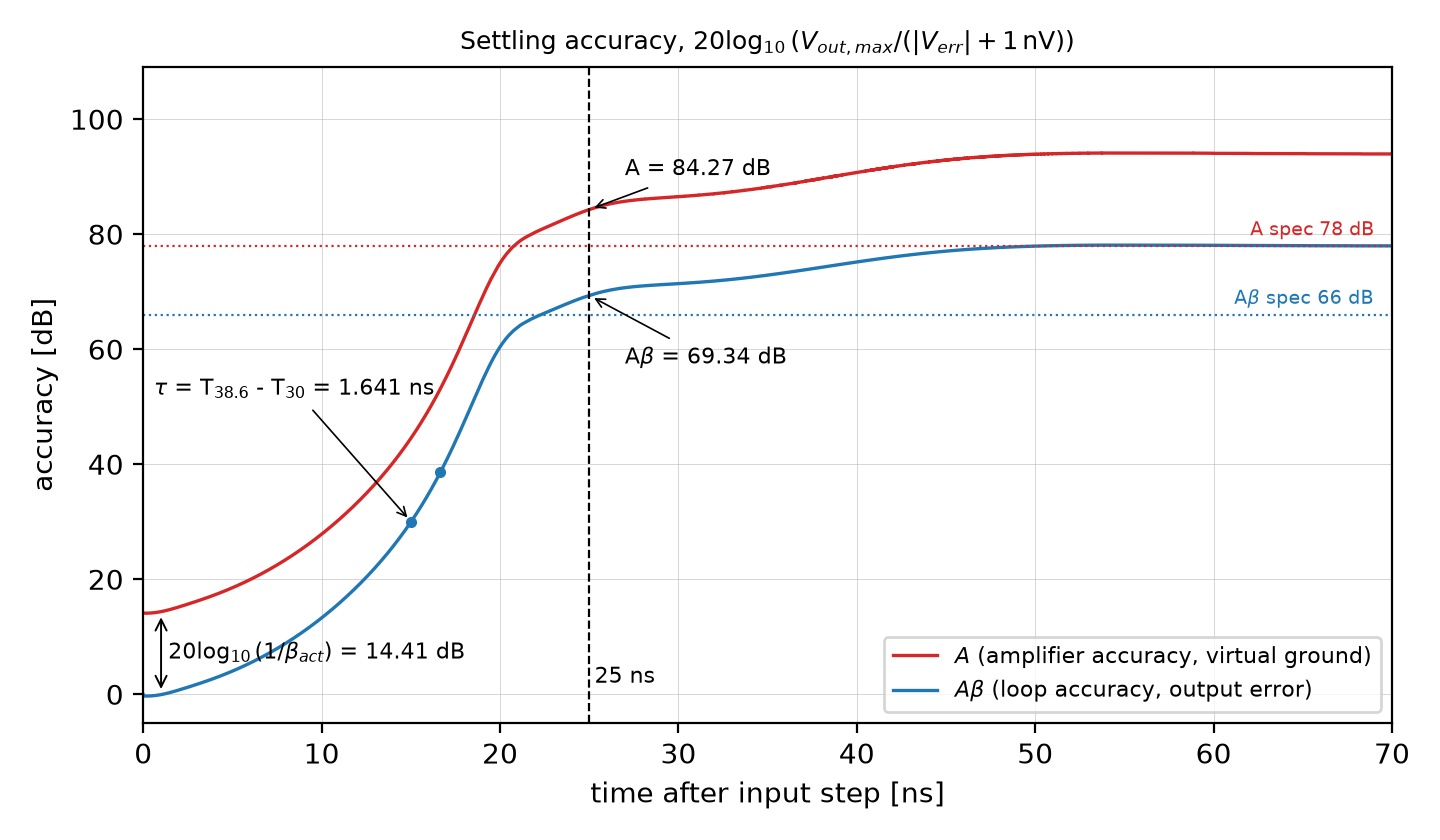
\includegraphics[width=\textwidth]{figures/d4_settling.png}
\fig{Deliverable 4: $A(t)$ and $A\beta(t)$ in ONE figure, $A\beta$ starting from 0\,dB, markers at 25\,ns / 78\,dB / 66\,dB}
\caption{Settling accuracy $A(t)$ and $A\beta(t)$ vs.\ time. The $A$--$A\beta$ gap is
$20\log_{10}(C_{in}/C_{fb})=12$\,dB.}
\end{figure}
At $t=25$\,ns: $A\beta_{\text{settle}}\ge 66$\,dB and $A_{\text{settle}}>78$\,dB. First ringing
peak (if any) appears after 25\,ns; up to two ringing cycles are acceptable.
\clearpage

% ============================== DELIVERABLE 5 ==============================
\section{Deliverable 5 -- Output Noise Power Density Versus Frequency}
\begin{figure}[H]\centering
% 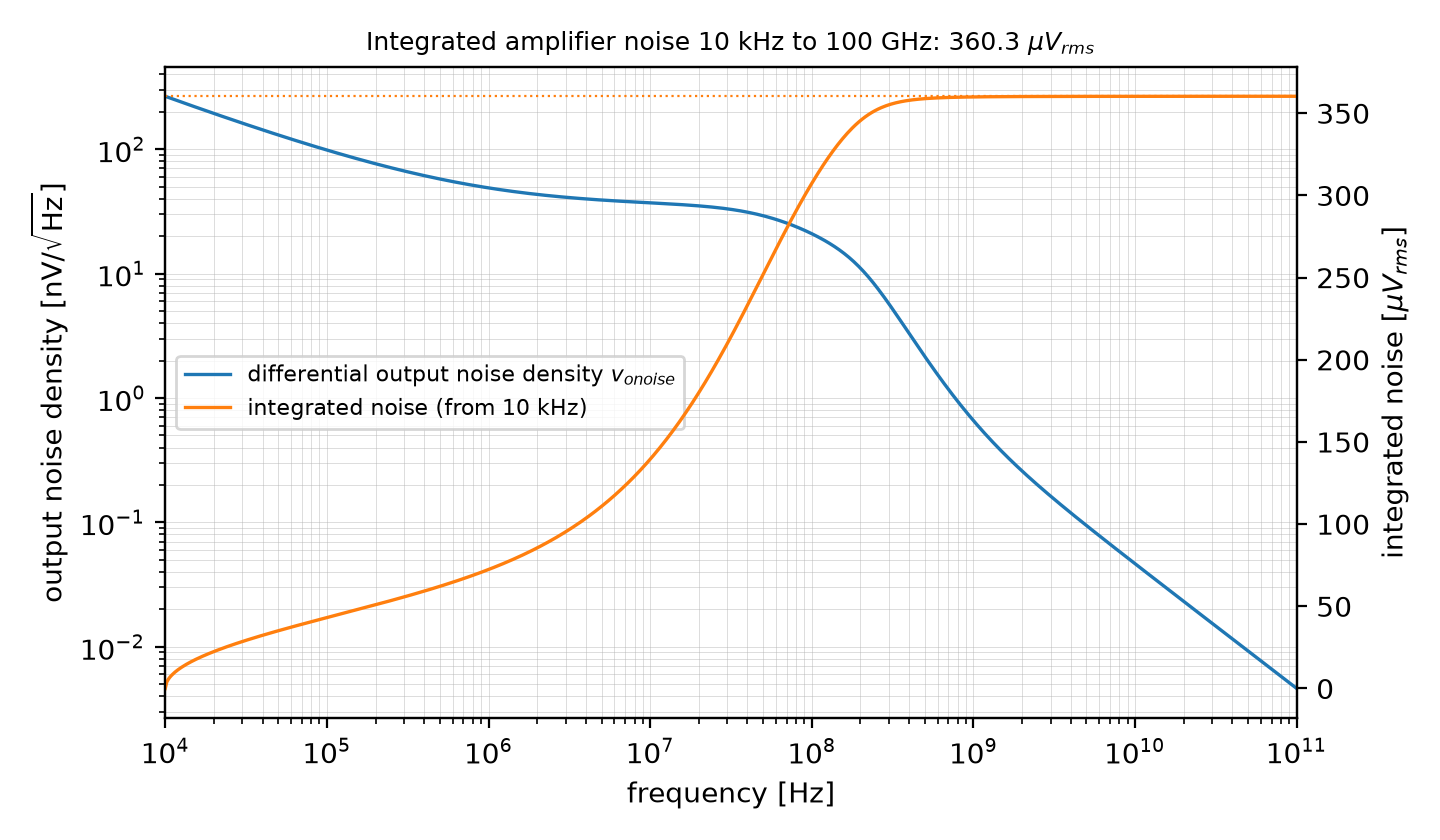
\includegraphics[width=\textwidth]{figures/d5_noise.png}
\fig{Deliverable 5: output-noise PSD 10\,kHz--100\,GHz with the integrated value shown}
\caption{Differential output-noise density vs.\ frequency, integrated 10\,kHz--100\,GHz.}
\end{figure}
Integrated amplifier noise $V_{n,amp}=\;$\rule{1.5cm}{0.4pt}$\;\mu$V$_{rms}$; adding the
hand-computed $kT/C$ (from $C_{in},C_{fb},C_{load}$ only) gives $V_{n,tot}$ and SNR $=$
\rule{1.2cm}{0.4pt}\,dB $\ge 66$\,dB.
\clearpage

% ============================== DELIVERABLE 6 ==============================
\section{Deliverable 6 -- FoM Comparison: EE4520 vs.\ EE4525}
Step-by-step explanation of the FoM difference (we took EE4520).
\begin{table}[H]\centering
\begin{tabular}{@{}l c c@{}}
\toprule
Quantity & EE4520 & EE4525 (this work) \\
\midrule
SNR [dB] & 80.85 & \\
$\tau$ [ns] & 497.4 & \\
Power [mW] & 0.1119 & \\
FoM$_{dB}$ [dB] & 175.20 & \\
\bottomrule
\end{tabular}
\end{table}
\noindent Discuss the main reasons the FoM differs (real CMFB/gain-boosters vs.\ ideal;
$1/f$ noise model; the much faster 25\,ns settling vs.\ 2.8\,$\mu$s; relaxed SNR; the
$\eta_{gm}/\mathrm{NEF}/\eta_{cur}/\eta_{vol}$ levers --- see \texttt{analysis/08\_power\_prediction.md}).
\clearpage

% ============================ SHORT EXPLANATION ============================
\section*{Short Explanation}
\addcontentsline{toc}{section}{Short Explanation}
% Max one page. Must EXPLAIN EVERY ASPECT OF THE D4 SETTLING PLOT, plus the bullets below.
\textbf{The settling plot (Deliverable 4).} [Explain the $A(t)$/$A\beta(t)$ shapes, the
$1/\beta$ gap, and why both meet 78/66\,dB at 25\,ns.]

\begin{itemize}
\item \textbf{Architecture + CMFB.} Single-stage gain-boosted cascode + current-reuse
      input; real switched-capacitor CMFB. [Why --- see \texttt{analysis/02}.]
\item \textbf{Sizing for noise (incl.\ $1/f$) and settling; output swing + capacitor sizing.}
      [\texttt{analysis/03}, \texttt{04}, \texttt{01}.]
\item \textbf{Dominant noise devices + NEF estimate.} [\texttt{analysis/04}.]
\item \textbf{Biasing.} [EE4520 bias block on a separate $V_{ddb}$; \texttt{analysis/01}.]
\end{itemize}
\clearpage

% ============================== APPENDIX ==============================
\appendix
\section{Appendix -- Simulation Schematics}
% Optional: the LTspice simulator schematics (render_schematic output), NOT D2/D3.
\begin{figure}[H]\centering
% \includegraphics[width=\textwidth]{figures/appendix_ac.png}
\fig{Appendix: LTspice testbench schematics (AC / transient / noise)}
\caption{Simulation testbenches.}
\end{figure}

\end{document}
